
\newcommand{\ee}{\ensuremath{\varepsilon}}

V predchádzajúcich častiach sme si ukázali simplexovú metódu na riešenie úlohy lineárneho programovania.
Povedali sme o nej, že je ''efektívna'', aj keď počet iterácií môže byť v najhoršom prípade 
exponenciálny od počtu premenných a obmedzení. V tejto kapitole si ukážeme inú metódu na riešenie
lineárnych programov, ktorá bude polynomiálna od veľkosti vstupu (viac o tom neskôr). Hlavný dôvod,
pre ktorý ju tu uvádzame, však nie je jej polynomialita, ale iné zaujímavé vlastnosti, ktoré takisto
uvidíme neskôr. Začnime zdanlivo nesúvisiacou geometrickou úlohou:

\begin{framed}
  \begin{dfn}
    \label{dfn:2dmember}
    V rovine je daný konvexný útvar $S$, ktorý celý leží v jednotkovom kruhu a má plochu aspoň \ee.
    Cieľom problému \member je nájsť nejaký bod z $S$.
  \end{dfn}
\end{framed}


\noindent
\begin{minipage}[t]{0.5\textwidth}
  \vskip 0pt
  Skúsme problém \member riešiť zovšeobecneným binárnym vyhľadávaním: začneme s jednotkovým kruhom. Ak jeho
  stred leží v $\cal S$, našli sme bod z $\cal S$. Inak z konvexnosti $S$ vieme, že existuje
  priamka prechádzajúca cez stred, ktorá rozdelí kruh na dve polovice tak, že
  $\cal S$ je v jednej z nich (na obrázku vpravo modrý polkruh).  
  Chceli by sme rekurzívne pokračovať v hľadaní iba v modrom
  polkruhu; problém je ale v tom, že postupne po veľa deleniach budeme dostávať
  stále zložitejšie útvary, ktoré si bude treba pamätať.  
  Ukáže sa, že dobrým riešením je zapamätať si najmenšiu elipsu opísanú modrému polkruhu (červená elipsa vpravo):
  je síce trocha väčšia, ako polkruh, ale (ako ukážeme) 
  stále menšia, ako pôvodný kruh. Keďže $S$ leží celý vovnútri elipsy,
  môžme našu úvahu zopakovať: ak 
\end{minipage}
\begin{minipage}[t]{0.5\textwidth}
  \vskip 0pt
\begin{center}
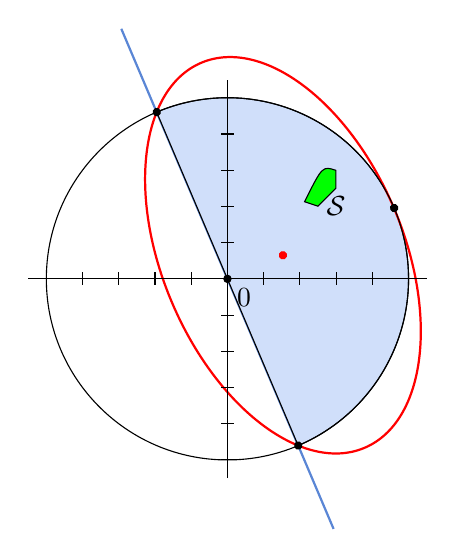
\begin{tikzpicture}[scale=2.3]

\begin{scope}[rotate=-157]
  \draw[draw=CornflowerBlue!90!black,thick] (0,-1.5) -- (0,1.5);
  \filldraw[ rotate=180, fill=CornflowerBlue!30, fill opacity=95] (0,-1) arc [start angle=-90, end angle=90, radius=1] -- cycle;
\draw[thick,draw=red] (-0.333,0) circle [x radius=0.666, y radius=1.1547];
\filldraw[red] (-0.333,0) circle [radius=0.02];

%\begin{scope}[shift={(-0.333,0)}]
%\draw[dashed, Salmon,  rotate=50] (0,-1.5) -- (0,1.5);
%\end{scope}

\filldraw (0,1) circle [radius=0.02];
\filldraw (0,-1) circle [radius=0.02] ;
\filldraw (-1,0) circle [radius=0.02] ;
\end{scope}
\filldraw[shift={(0.5,0.5)}, scale=0.07, rotate=45, draw=black, fill=green] 
      (-1,-1) -- (1,-1) -- (2,0) .. controls (1.5,1)  ..  (-1.5,0) -- cycle;
      \draw (0.6,0.4) node {$\cal S$};
\draw (0,0) circle [radius=1] node[anchor=north west] {$0$};
\filldraw (0,0) circle [radius=0.02];
%axis
\draw (-1.1,0) -- coordinate (x axis mid) (1.1,0);
\draw (0,-1.1) -- coordinate (y axis mid) (0,1.1);
%ticks
\foreach \x in {-1,-0.8,...,1}
\draw (\x,1pt) -- (\x,-1pt);
\foreach \y in {-1,-0.8,...,1}
\draw (1pt,\y) -- (-1pt,\y);

\end{tikzpicture}
\end{center}
\end{minipage}
\noindent  
  stred elipsy leží v $S$, 
  máme riešenie, inak 
  opäť existuje priamka prechádzajúca stredom elipsy tak, 
  že $S$ je v jednej polovici; môžeme nájsť najmenšiu
  elipsu opísanú príslušnej ''polelipse'' a takto pokračovať ďalej.
Pripomeňme, že elipsa $E$ so stredom v bode $(0,0)$ a jej plocha $\lVert E\rVert$ sú dané nasledovnými vzťahmi,
pričom $a$, $b$ sú dĺžky jednotlivých poloosí:

\begin{minipage}[t]{0.5\textwidth}
  \vskip 0pt
\begin{center}
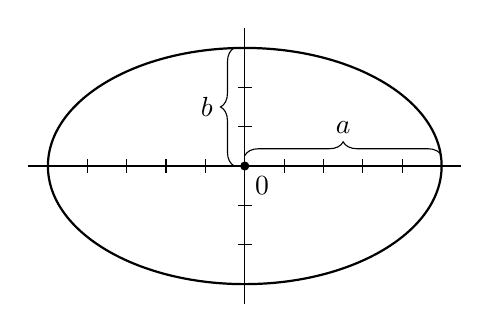
\begin{tikzpicture}[scale=2.5]

  \draw[thick] (0,0) ellipse (1.0 and 0.6)  node[anchor=north west] {$0$};
\filldraw (0,0) circle [radius=0.02];
%axis
\draw (-1.1,0) -- coordinate (x axis mid) (1.1,0);
\draw (0,-0.7) -- coordinate (y axis mid) (0,0.7);

 \draw [decorate,decoration={brace,amplitude=5pt,raise=5pt},xshift=0pt,yshift=-0.5pt] (0,0) -- (1,0)
  node[black,midway,yshift=15pt] {$a$};
 
  \draw [decorate,decoration={brace,amplitude=5pt,raise=5pt},xshift=0.5pt,yshift=0pt] (0,0) -- (0,0.6)
  node[black,midway,xshift=-15pt] {$b$};

%ticks
\foreach \x in {-1,-0.8,...,1}
\draw (\x,1pt) -- (\x,-1pt);
\foreach \y in {-0.6,-0.4,...,0.6}
\draw (1pt,\y) -- (-1pt,\y);


\end{tikzpicture}
\end{center}
\end{minipage}
\begin{minipage}[t]{0.5\textwidth}
  \vskip 0pt
  \begin{eqnarray*}
    E &=& \left\{ (x,y)\in\R^2\mid \frac{x^2}{a^2}+\frac{y^2}{b^2}\le1\right\} \\
    \lVert E\rVert & =& \pi a b
    \end{eqnarray*}
\end{minipage}


\noindent
Aby náš postup zafungoval, musíme vedieť nájsť najmenšiu elipsu opísanú generickej polelipse a ukázať, že jej plocha 
je o konštantný faktor menšia. Majme teda elipsu v ľubovoľnej polohe a priamku prechádzajúcu jej stredom. 
Začneme tým, že elipsu presunieme do bodu
$(0,0)$ a otočíme tak, aby jej osi boli rovnobežné so súradnicovými osami. 


\begin{minipage}[t]{0.5\textwidth}
  \vskip 0pt
\begin{center}
\begin{tikzpicture}[scale=2.5]


\end{tikzpicture}
\end{center}
\end{minipage}
\begin{minipage}[t]{0.5\textwidth}
  \vskip 0pt
\begin{center}
\begin{tikzpicture}[scale=2.5]

\end{tikzpicture}
\end{center}
\end{minipage}


\IGNORE{
\vspace*{-4ex}
\noindent
\colorlet{shadecolor}{Aquamarine!9}
\begin{shaded}
\subsection*{Malá odbočka k elipsám}

\noindent
Čitateľ sa už možno stretol s konvexným obalom v dvoch rozmeroch: pre dané body
v rovine je ich konvexný obal najmenší konvexný mnohouholník, ktorý ich všetky obsahuje.

\end{shaded}



  elipsa opísaná polkruhu. Pozrime sa preto na elipsu trocha bližšie. Čitateľ si azda pamätá, že elipsa\footnote{% 
keď budeme hovoriť o elipse, vždy budeme myslieť elipsu aj s vnútrom} 
stredom v $[0,0]$ a poloosami $a$, $b$ je množina bodov $[x,y]$ v rovine, spĺňajúcich vzťah
$$\frac{x^2}{a^2}+\frac{y^2}{b^2}\le1$$
a jej plocha je $\pi ab$.

\begin{center}
\begin{tikzpicture}[scale=2.3]

% elipsa
\begin{scope} [rotate=-157]
\end{scope}


\end{tikzpicture}
\end{center}
}
